\section{Unit Testing}
\label{unitTesting}
In this section, a description of the unit tests, which were constructed in an effort to check the quality and correctness of the software solution described in this report, will be presented.

\subsection{What is Unit Testing?}
Unit testing is a way of dividing code into small portions, which can then independently be tested for correctness\cite{unittesting}.

Unit tests should be quick, meaning that a developer can verify whether or not the code is correct, during development, without having to disrupt his work flow, to wait for the results.
Unit tests should also be small, checking only a single or very small subset of the functionality of the systems code.
Lastly, and perhaps most importantly, unit tests should be correct. If a unit test gives a false positive\footnote{A \emph{false positive} is when a test indicates that a condition is true, when, in reality, the condition is false. Likewise, a \emph{false negative} is when a test indicates a condition being false, when it is true.} then a developer would likely be convinced that the code which has been produced is working as it should, when in reality it is not. This could potentially lead to a logical error breaking the application on the end users' devices, among other undesirable situations. Likewise, if a unit test gives a false negative, a developer could waste a lot of time refactoring code, rewriting algorithms and modifying logic, even though the code was correct.

\subsection{Unit Testing for openPlaylist}
Unit testing in the system described in this report was implemented mostly on the server side. This was done, as the server side of openPlaylist is much more extensive than the rather dumb client.
The unit tests which were implemented covered various parts of the code, some test the correctness of methods, others verify connections to third party servers and some verify type extensions.
Unit tests for this project were implemented using xUnit.net\footnote{\url{http://xunit.github.io/}}, a powerful tool set for building unit tests in the .Net framework. In xUnit.net, most unit tests are created using assertions, which check that a certain condition is met and if not, fails the test.
To run the unit tests, a developer simply has to click the \enquote{Run All}-button in the Test Explorer in Visual Studio. This gives the developer a quick overview of the unit tests and whether or not they have passed, as can be seen in \cref{fig:UnitTestsPassed}.

\begin{figure}[H]
  \centering
  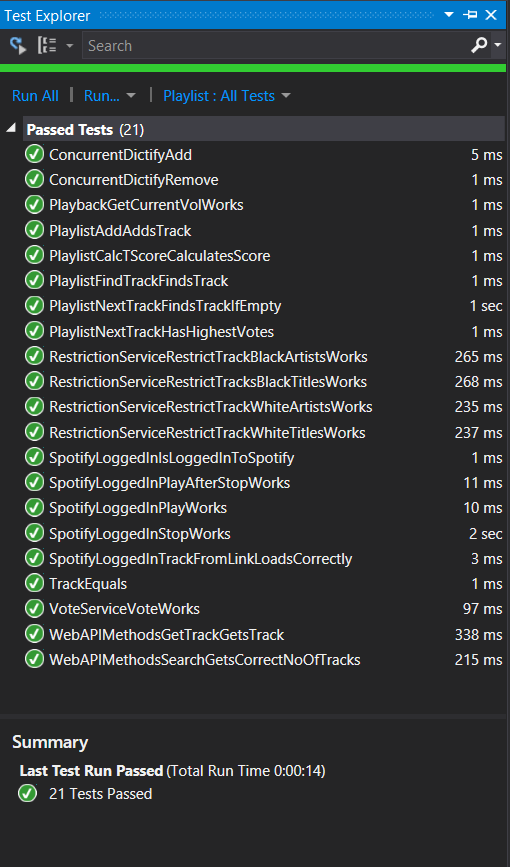
\includegraphics[width=.7\textwidth]{UnitTestsPassed.png}
  \caption{The Test Explorer in Visual Studio.}\label{fig:UnitTestsPassed}
\end{figure}

As can be seen in \cref{lst:UnitTest}, the unit tests which were implemented in the software solution were fairly simple. The example shows the manual creation of a \emph{Track} and a call to a method, which will automatically get the \emph{Track}. The test is simply an assertion that the two \emph{Track}s are identical. In \cref{fig:UnitTestsPassed}, it can be seen that this assertion is indeed true and the test has passed. This should mean that the method for automatically getting a \emph{Track} works as it should.
It should be noted that the method for getting a \emph{Track} uses a third party database. This means that, in a situation where the database has modified the data for this particular \emph{Track}, the test would fail, as it would not be equal to the manually constructed \emph{Track}. However, if the test passes, it is extremely unlikely that the method, which is tested, is incorrect.

\begin{lstlisting}[float, floatplacement=htpb,caption = {Test method for the automatic getting of a \textbf{Track}}, label = {lst:UnitTest}]
[Fact]
public void WebAPIMethodsGetTrackGetsTrack()
{
	(...)
	var track = new Track("19pTAbMZmWsgGkYZ4v2TM1", "Obliteration of the Weak", 232120, false, 1, "DKFD51642001" , "https://p.scdn.co/mp3-preview/1d3ee1111d679b5e5b50c53aa3bfcceb4c83da8a", alb);

	var foundTrack = WebAPIMethods.GetTrack(track.URI);

	Assert.Equal(track, foundTrack);
}
\end{lstlisting}
